\chapter{Methodology}

To keep track of version control, the code is version controlled using GitHub \cite{dissertaiton_github}.

\section{Agile methodology}

The project was undertaken using an agile methodology. This was to allow for development and revision rather than using the waterfall model which requires all the planning to be done upfront. Waterfall requires all the planning of what will be done and when it will be done without any change. Then in development, everything has to be done from start to finish and shipped. There is no changing of mind during development.

Agile development allows for the project to change as it is being developed if needed. It means the requirements can be gathered, planned out and develop much quicker as it is not set in stone, the requirements can change over time if needed.

\subsection{Kanban}

Tracking what needs to be done on the project and what has already been done is a very important task as it allows for the tracking of whether the project is on track, and helps to determine what features can be worked on given the time frame remaining.

\begin{figure}[H]
    \centering
    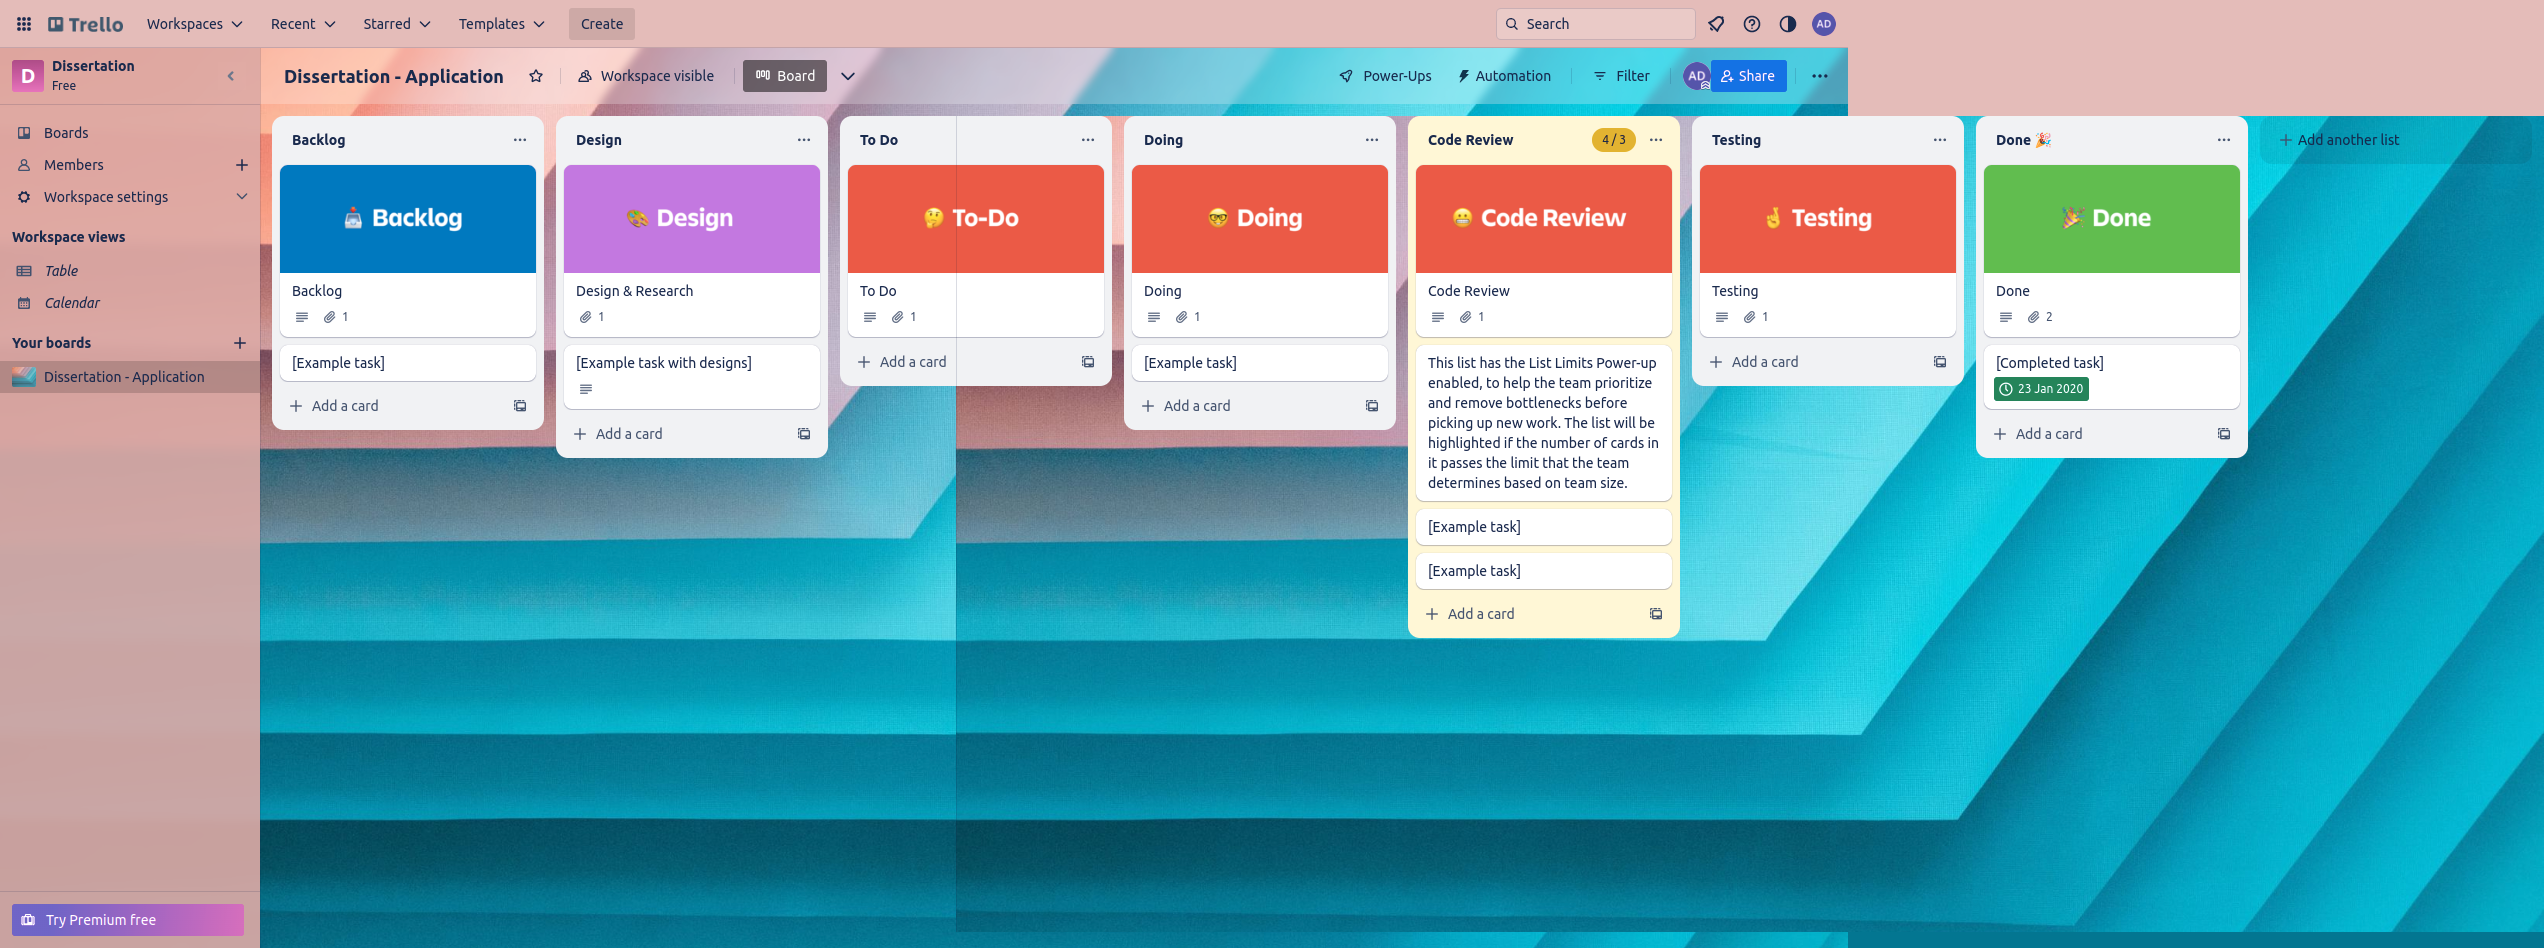
\includegraphics[scale=0.15]{images/starting trello.png}
    \caption{Trello as the Kanban tracker}
    \label{fig:my_label}
\end{figure}


\begin{figure}[H]
    \centering
    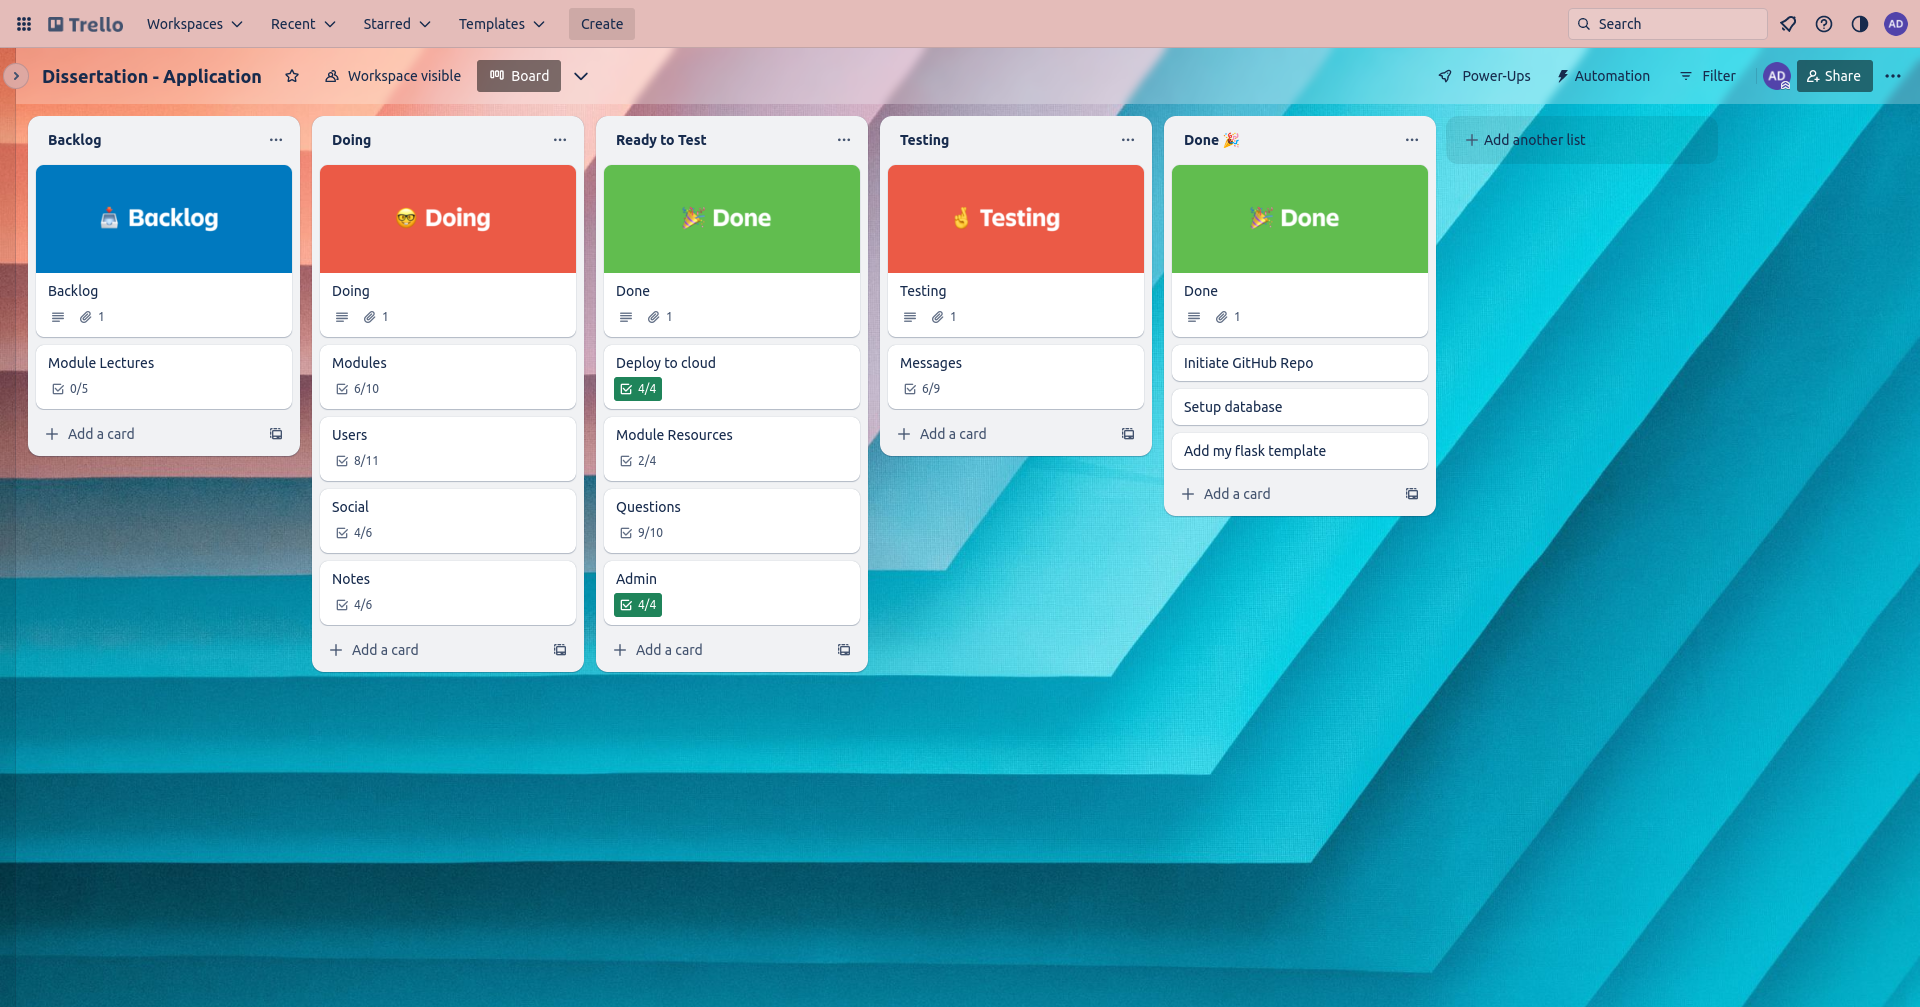
\includegraphics[scale=0.20]{images/trello_final.png}
    \caption{The final view of Trello after project completion}
    \label{fig:my_label}
\end{figure}

\section{Tools}

\subsection{Tools used}

For developing and deploying the application, a variety of tools were used. AWS (Amazon Web Services) was used to host the Database and web application, ImageKit for the Image and PDF storage, git/GitHub for version control, Trello for project tracking, ChatGTP for questions (and search engine) and VS Code as the IDE (Integrated Development Environment) of choice.

\subsubsection{AWS}

Amazon Web Services (AWS) is a cloud hosting platform which allows someone to rent server space along with many other back-end services. AWS was used to host the application instead of needing to buy and deploy servers.

\subsubsection{ImageKit}

ImageKit was used for storing and delivering the photos and pdfs which users upload through the application using module resources.

\subsubsection{git + GitHub}

GitHub along with git was used for version control for the project's codebase. It allows for the code to be saved and uploaded to the cloud keeping a history of the code changes every time code is pushed to GitHub.

\subsubsection{Trello}

Trello was the program of choice for tracking the progress of the project using Kanban. GitHub is a good and probably better option as it has a built-in Kanban tracker which when taken full advantage of is very powerful even allowing for stories and issues to automatically be completed with code pushes. Trello was used for simplicity and due to already familiarity with the application.

\subsubsection{VS Code}
VS Code was used as the ide code editor of choice.